
%------------------------------------------------------------
\begin{ex}%[2D4V3-4]%Câu 1.
\immini{Có một cốc nước thủy tinh hình trụ, bán kính trong lòng đáy cốc là $6\,\text{cm}$, chiều cao lòng cốc là $10\,\text{cm}$ đang đựng một lượng nước. Tính thể tích lượng nước trong cốc, biết khi nghiêng cốc nước vừa lúc khi nước chạm miệng cốc thì đáy mực nước trùng với đường kính đáy.
\choice
{\True $240$\,cm$^3$}
{$240\pi$ \,cm$^3$}
{$120$\,cm$^3$}
{$120\pi$ \,cm$^3$}}
{\begin{tikzpicture}[scale=0.7, font=\footnotesize,line join=round, line cap=round, >=stealth]
\begin{scope}[shift={(0,0)}]
	\def\a{1.5}
	\def\b{.5}
	\def\h{4}
	\path
	(0,0) coordinate (M)
	($(M)+(2*\a,0)$) coordinate (N)
	($(M)!0.5!(N)$)coordinate (O)
	($(M)+(0,\h)$) coordinate (M')
	($(N)+(0,\h)$) coordinate (N')
	($(O)+(0,\h)$) coordinate (O')
	($(M')!0.6!(M)$)coordinate (A)
	($(N')!0.6!(N)$)coordinate (B)
	;
	\fill[black!15] (A) arc (180:0:\a cm and \b cm)--(N)--(M) arc (-180:0:\a cm and \b cm)--(M)--(A);
	\draw(M)--(M') (N)--(N');
	\draw[dashed,thin] (M) arc (180:0:\a cm and \b cm);
	\draw[dashed,thin] (A) arc (180:0:\a cm and \b cm);
	\draw (O') ellipse (\a cm and \b cm)	(M) arc (-180:0:\a cm and \b cm) (A) arc (-180:0:\a cm and \b cm);
\end{scope}
\begin{scope}[rotate=-70,shift={(0,6)}]
	\def\a{1.5}
	\def\b{.5}
	\def\h{4}
	\path
	(0,0) coordinate (M)
	($(M)+(2*\a,0)$) coordinate (N)
	($(M)!0.5!(N)$)coordinate (O)
	($(M)+(0,\h)$) coordinate (M')
	($(N)+(0,\h)$) coordinate (N')
	($(O)+(0,\h)$) coordinate (O')
	($(M')!0.6!(M)$) coordinate (A)
	($(N')!0.6!(N)$) coordinate (B)
	;
	\fill[black!15]  (2.1,-.45)--(.8,.45) .. controls +(70:2) and +(180:0) ..(N') (N').. controls +(-90:.3) and +(180:0) ..(N).. controls +(-90:.3) and +(0:0.3) ..(2.1,-.45);
	\draw(M)--(M') (N)--(N');
	\draw[dashed,thin] (M) arc (180:0:\a cm and \b cm);
	\draw (O') ellipse (\a cm and \b cm)	(M) arc (-180:0:\a cm and \b cm);

	\draw[dashed] (2.1,-.45)--(.8,.45) .. controls +(70:2) and +(180:0) ..(N') (1.5,0)--(N');
	\draw (2.1,-.45) .. controls +(40:1) and +(180:0) ..(N') ;
	
\end{scope}
\end{tikzpicture}} 

\loigiai{
\textbf{Cách 1.} 
\begin{center}
\begin{tikzpicture}[scale=1, font=\footnotesize,line join=round, line cap=round, >=stealth]
	\path
		(0,0) coordinate (A)
		(0,3) coordinate (B)
		;
	
	\draw (A) arc (0: -90: 5 and 2) coordinate (C);
	\draw[dashed] (A) arc (0: 90: 4.5 and 2) coordinate (D);
	\coordinate (I) at ($(C)!.5!(D)$);
	\draw (A)--(B) (C)--(D) (I)--(B);
	\draw[dashed] (I)--(A);
	\draw 
	(C) .. controls +(0:0) and +(-90:1.5) ..(B).. controls +(90:1.5) and +(60:0) ..(D);
	\draw pic[draw, angle radius=2mm]{right angle=B--A--I};
	\pic[draw,"$\alpha$", angle eccentricity=0.6,angle radius=0.8cm]{angle=A--I--B};
	\path (A)--(I) node[above,pos=.7,sloped]{$R$};
	\path (C)--(I) node[above,midway,sloped]{$R$};
	\path (D)--(I) node[above,midway,sloped]{$R$};
\end{tikzpicture}
\end{center}
Xét thiết diện cắt cốc thủy tinh vuông góc với đường kính tại vị trí bất kỳ có  
$$S(x)=\dfrac{1}{2}\sqrt{R^2-x^2}\cdot \sqrt{R^2-x^2}\cdot \tan \alpha= \dfrac{1}{2}\left( R^2-x^2 \right)\tan \alpha.$$
Thể tích hình cái nêm là: $V=\dfrac{1}{2}\tan \alpha \displaystyle\int\limits_{-R}^{R}{\left( R^2-x^2 \right)}\text{d}x=\dfrac{2}{3}R^3\tan \alpha $.\\
Thể tích khối nước tạo thành khi nguyên cốc có hình dạng cái nêm nên $V_{kn}=\dfrac{2}{3}R^3\tan \alpha $. \\
$\Rightarrow V_{kn}=\dfrac{2}{3}R^3\cdot \dfrac{h}{R}=240\,cm^3$.\\
\textbf{Cách 2.} 
\begin{center}
\begin{tikzpicture}[scale=1, font=\footnotesize,line join=round, line cap=round, >=stealth]
	\path
	(0,0) coordinate (O)
	(0,4) coordinate (O')
	(7,0) coordinate (J)
	(7,4) coordinate (J')
	(9,0) coordinate (x)
	($(J)!.5!(J')$) coordinate (I)
	($(O)!.5!(O')$) coordinate (I')
	;
	\fill[cyan!20] (J)--(O) .. controls +(82:0.6) and +(180:0.6) ..
	(6.15,3.15)--(7.85,.9).. controls +(180:0.05) and +(0:.6) ..
	(7,0);
	\draw[->] (O)--(x);
	\draw[dashed,name path=OB] 
	(O) .. controls +(82:0.6) and +(180:0.6) ..
	(6.15,3.15)coordinate (B)--(7.85,.9) coordinate (A);
	\draw (0,2) ellipse (1 and 2) (O)--(O') (O')--(J') ;
	\draw (J) arc (-90: 90: 1 and 2);
	\draw[dashed] (J) arc (-90: 90: -1 and 2) (J)--(J') ;
	\draw[dashed,name path=II'] (I)--(I');
	\path [name intersections={of=OB and II',by=H}];
	\coordinate (E) at ($(J)!(H)!(O)$);
	\coordinate (N) at ($(O)!.55!(A)$);
	
	\path (intersection of H--E and O--I) coordinate (F);
	\coordinate (n) at ($(F)!-3!(N)$);
	\path[name path=FN] (N)--(n);
	\path [name intersections={of=OB and FN,by=M}];
	
	\fill[orange!50] (M) .. controls +(-90:1) and +(180:.5) ..(E) .. controls +(0:.5) and +(180:0) ..(N);
	\draw[dashed] (H)--(E) (M)--(N) (H)--(N) (O)--(I);
	\draw[dashed] (M) .. controls +(-90:1) and +(180:.5) ..(E);
	\draw (E) .. controls +(0:.5) and +(180:0) ..(N) (O)--(A);
	\draw[<->] ($(O)+(0,-.3)$)--($(E)+(0,-.3)$) node[fill=white,midway,sloped]{$x$};
	\draw[<->] ($(O')+(0,.3)$)--($(J')+(0,.3)$) node[fill=white,midway,sloped]{$10$ cm};
	\draw[<->] ($(J)+(1.5,0)$)--($(J')+(1.5,0)$) node[fill=white,midway,sloped]{$12$ cm};
	\draw[->] ($(E)+(.5,.3)$)--($(E)+(.8,-.5)$) node[below] {$S(x)$};
	\pic[draw,"$\alpha$", angle eccentricity=1.1,angle radius=2cm]{angle=J--O--I};
	\node[above right] at (F) {$\beta$};
	\foreach \x/\g in {H/90,E/-70,F/120,N/-90,M/90,I/0,J/-90,O/-120} \fill[black] (\x) circle (1pt)+(\g:.3) node {$\x$};
\end{tikzpicture}
\end{center}
Dựng hệ trục tọa độ $Oxyz$.\\
 Gọi $S\left( x \right)$ là diện tích thiết diện do mặt phẳng có phương vuông góc với trục $Ox$ với khối nước, mặt phẳng này cắt trục $Ox$ tại điểm có hoành độ $h\ge x\ge 0$.\\
Gọi $\widehat{IOJ}=\alpha ,\,\widehat{FHN}=\beta ,\,OE=x$\\
$\tan \alpha =\dfrac{IJ}{OJ}=\dfrac{6}{10}=\dfrac{EF}{OE}\Rightarrow EF=\dfrac{6x}{10}\Rightarrow HF=6-\dfrac{6x}{10}$.\\
$\cos \beta =\dfrac{HF}{HN}=\dfrac{6-\dfrac{6x}{10}}{6}=1-\dfrac{x}{10}\Rightarrow \beta =\arccos \left( 1-\dfrac{x}{10} \right)$\\
%-------------------------------------
$S\left( x \right)=S_{\text{hình quạt}}-S_{HMN}=\dfrac{1}{2}HN^2\cdot 2\beta -\dfrac{1}{2}HM\cdot HN\cdot \sin 2\beta $\\
%-------------------------------------
$\Rightarrow S\left( x \right)=6^2\arccos \left( 1-\dfrac{x}{10} \right)-\dfrac{1}{2}\cdot 6\cdot 6\cdot 2\left( 1-\dfrac{x}{10} \right)\sqrt{1-\left( 1-\dfrac{x}{10} \right)^2}$\\
$\Rightarrow V=\displaystyle\int\limits_{0}^{10}{S\left( x \right) \,\mathrm{d}x}=\displaystyle\int\limits_{0}^{10}{\left( 36\arccos \left( 1-\dfrac{x}{10} \right)-36\left( 1-\dfrac{x}{10} \right)\sqrt{1-\left( 1-\dfrac{x}{10} \right)^2} \right)\,\mathrm{d}x}=240$.}
\end{ex}
%------------------------------------------------------------
\begin{ex}%[2D4V3-4]%Câu 2.
\immini{Cho vật thể đáy là hình tròn có bán kính bằng 1 (tham khảo hình vẽ). Khi cắt vật thể bằng mặt phẳng vuông góc với trục $Ox$ tại điểm có hoành độ $x\ \left( -1\le x\le 1 \right)$ thì được thiết diện là một tam giác đều. Thể tích $V$ của vật thể đó là
\choice
{$V=\sqrt{3}$}
{$V=3\sqrt{3}$}
{\True $V=\dfrac{4\sqrt{3}}{3}$}
{$V=\pi $}}
{\includegraphics[scale=0.4]{image/Cau2_C4B3CD3.png} }
\loigiai{
\immini{
Do vật thể có đáy là đường tròn và khi cắt bởi mặt phẳng vuông góc với trục $Ox$ được thiết diện là tam giác đều do đó vật thể đối xứng qua mặt phẳng vuông góc với trục $Oy$ tại điểm $O$.\\
Cạnh của tam giác đều thiết diện là  $a=2\sqrt{1-x^2}$.\\
Diện tích tam giác thiết diện là  
$$S=\dfrac{a^2\sqrt{3}}{4}=\left( 1-x^2 \right)\sqrt{3}.$$
}
{\begin{tikzpicture}[scale=0.7, font=\footnotesize,line join=round, line cap=round, >=stealth]
	\path
	(0,0) coordinate (O)
	(60:3) coordinate (A)
	(-60:3) coordinate (B)
	($(A)!.5!(B)$) coordinate (x)
	;
	\draw (O) circle (3) (O)--(A)--(B);
	\draw[->] (-4,0) -- (4,0)node[below] {$x$};
	\draw[->] (0,-4) -- (0,4)node[right] {$y$};
	\path (A)--(B) node[above right,midway]{$\sqrt{1-x^2}$};
	\foreach \x/\g in {O/-120,x/-70} \fill[black] (\x) circle (1pt)+(\g:.3) node {$\x$};
\end{tikzpicture}}
\noindent
Thể tích khối cần tìm là 
$$V=2\displaystyle\int\limits_{0}^{1}{Sdx}=2\displaystyle\int\limits_{0}^{1}{\sqrt{3}\left( 1-x^2 \right)=\left. 2\sqrt{3}\left( x-\dfrac{x^3}{3} \right) \right|_{0}^{1}=\dfrac{4\sqrt{3}}{3}}.$$
}
\end{ex}
%------------------------------------------------------------
\begin{ex}%[2D4V3-4]%Câu 3.
Sân vận động Sport Hub (Singapore) là sân có mái vòm kỳ vĩ nhất thế giới. Đây là nơi diễn ra lễ khai mạc Đại hội thể thao Đông Nam Á được tổ chức tại Singapore năm $2015$. Nền sân là một elip $\left( E \right)$ có trục lớn dài $150m$, trục bé dài $90m$ (hình vẽ). Nếu cắt sân vận động theo một mặt phẳng vuông góc với trục lớn của $\left( E \right)$và cắt elip ở $M,N$ (hình vẽ) thì ta được thiết diện luôn là một phần của hình tròn có tâm $I$ (phần tô đậm trong hình 4) với $MN$ là một dây cung và góc $\widehat{MIN}=90^{\circ}.$ Để lắp máy điều hòa không khí thì các kỹ sư cần tính thể tích phần không gian bên dưới mái che và bên trên mặt sân, coi như mặt sân là một mặt phẳng và thể tích vật liệu là mái không đáng kể. Hỏi thể tích xấp xỉ bao nhiêu?
  \begin{center}
  {\includegraphics[scale=0.8]{image/Cau3_C4B3CD3.png}\\
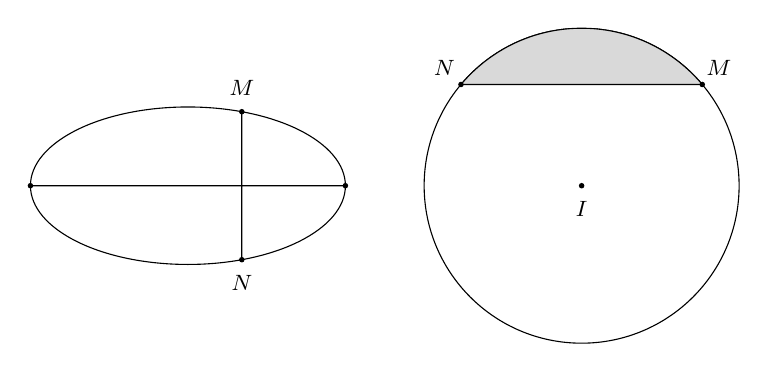
\begin{tikzpicture}[scale=1, font=\footnotesize,line join=round, line cap=round, >=stealth]
	\path
	(0,0) coordinate (O)
	(-2,0) coordinate (A)
	(2,0) coordinate (B)
	(70: 2 and 1) ellipse  coordinate (M)
	(-70: 2 and 1) ellipse  coordinate (N)
	;
	\draw (O) ellipse (2 and 1) (M)--(N) (A)--(B);
	\fill[black] (B) circle (1pt);
	\fill[black] (A) circle (1pt);
	\foreach \x/\g in {M/90,N/-90} \fill[black] (\x) circle (1pt)+(\g:.3) node {$\x$};
	\begin{scope}[shift={(5,-0)}]
		\path (0,0) coordinate (I) (40:2)   coordinate (M)
		(140:2)  coordinate (N) ;
		\draw (I) circle (2) (M)--(N);
		
		
		\clip (-2,1.28) rectangle (2,2);
		\fill[black!15] (I) circle (2);
		\draw (I) circle (2) (M)--(N);
	\end{scope}
	\foreach \x/\g in {M/45,N/135,I/-90} \fill[black] (\x) circle (1pt)+(\g:.3) node {$\x$};
\end{tikzpicture} }
  \end{center}
\choice
{$57793$ m$^3$}
{\True $115586$ m$^3$}
{$32162$ m$^3$}
{$101793$ m$^3$}
\loigiai{
\begin{center}
\includegraphics[scale=0.8]{image/Cau3_C4B3CD3_g.png}
\end{center}
Chọn hệ trục như hình vẽ\\
Ta cần tìm diện tích của $S\left( x \right)$thiết diện.\\
Gọi $d\left( O,MN \right)=x$\\
$\left( E \right)\colon\dfrac{x^2}{75^2}+\dfrac{y^2}{45^2}=1.$\\
Lúc đó $MN=2y=2\sqrt{45^2\left( 1-\dfrac{x^2}{75^2} \right)}=90\sqrt{1-\dfrac{x^2}{75^2}}$\\
$\Rightarrow R=\dfrac{MN}{\sqrt{2}}=\dfrac{90}{\sqrt{2}}.\sqrt{1-\dfrac{x^2}{75^2}}\Rightarrow R^2=\dfrac{90^2}{2}\cdot \left( 1-\dfrac{x^2}{75^2} \right)$.\\
$S\left( x \right)=\dfrac{1}{4}\pi R^2-\dfrac{1}{2}R^2=\left( \dfrac{1}{4}\pi -\dfrac{1}{2} \right)R^2=\left( \pi -2 \right)\dfrac{2025}{2}.\left( 1-\dfrac{x^2}{75^2} \right).$\\
Thể tích khoảng không cần tìm là
$$V=\displaystyle\int\limits_{-75}^{75}\left( \pi -2 \right)\dfrac{2025}{2}.\left( 1-\dfrac{x^2}{75^2} \right)\approx 115586 \,\text{m}^3.$$
}
\end{ex}
%------------------------------------------------------------
\begin{ex}%[2D4V3-4]%Câu 4.
\immini{Gọi $\left( H \right)$ là phần giao của hai khối $\dfrac{1}{4}$ hình trụ có bán kính $a$, hai trục hình trụ vuông góc với nhau như hình vẽ sau. Tính thể tích của khối $\left( H \right)$.
\choice
{${{V}_{\left( H \right)}}=\dfrac{a^3}{2}$}
{${{V}_{\left( H \right)}}=\dfrac{3a^3}{4}$}
{\True $V_{\left( H \right)}=\dfrac{2a^3}{3}$}
{${{V}_{\left( H \right)}}=\dfrac{\pi a^3}{4}$}}
{\includegraphics[scale=0.8]{image/Cau4_C4B3CD3_De.png}}
\loigiai{
\begin{center}
\includegraphics[scale=0.8]{image/Cau4_C4B3CD3.png}
\end{center}
+ Đặt hệ toạ độ $Oxyz$ như hình vẽ, xét mặt cắt song song với mp $\left( Oyz \right)$ cắt trục $Ox$ tại $x$: thiết diện mặt cắt luôn là hình vuông có cạnh $\sqrt{a^2-x^2}$ $\left( 0\le x\le a \right)$.\\
+ Do đó thiết diện mặt cắt có diện tích: $S\left( x \right)=a^2-x^2$.\\
+ Vậy $V_{\left( H \right)}=\displaystyle\int\limits_{0}^{a}{S\left( x \right)\,\mathrm{\,d}x} =\displaystyle\int\limits_{0}^{a}{\left( a^2-x^2 \right)\,\mathrm{d}x} =\left. \left( a^2x-\dfrac{x^3}{3} \right) \right|_{0}^{a}$\\
$=\dfrac{2a^3}{3}$}
\end{ex}
%------------------------------------------------------------
\begin{ex}%[2D4H3-5]%Câu 5.
Một bác thợ xây bơm nước vào bể chứa nước. Gọi $h\left( t \right)$ là thể tích nước bơm được sau $t$ giây. Cho ${h}'\left( t \right)=6at^2+2bt$ và ban đầu bể không có nước. Sau 3 giây thì thể tích nước trong bể là $90m^3$, sau $6$ giây thì thể tích nước trong bể là $504m^3$. Tính thể tích nước trong bể sau khi bơm được $9$ giây.
\choice
{\True $1458m^3$}
{$600m^3$}
{$2200m^3$}
{$4200m^3$}
\loigiai{
$\displaystyle\int\limits_{0}^{3}\left( 6at^2+2bt \right)\,\mathrm{d}t=90\Leftrightarrow \left.\left( 2at^3+bt^2 \right) \right|_{0}^{3}=90\Leftrightarrow 54a+9b=90$\quad (1)\\
$\displaystyle\int\limits_{0}^{6}\left( 6at^2+2bt \right)\,\mathrm{d}t=504 \Leftrightarrow  \left. \left( 2at^3+bt^2 \right) \right|_{0}^{6}=504\Leftrightarrow 432a+36b=504$\quad (2)\\
Từ (1), (2) $\Rightarrow  \heva{
  & a=\dfrac{2}{3} \\ 
 & b=6.}$\\
Sau khi bơm $9$ giây thì thể tích nước trong bể là\\
$V=\displaystyle\int\limits_{0}^{9}\left(4t^2+12t \right)\,\mathrm{d}t =  \left. \left(\dfrac{4}{3}t^3+6t^2 \right) \right|_{0}^{9}=1458\; \left(m^3 \right)$.}
\end{ex}
%------------------------------------------------------------
\begin{ex}%[2D4H3-5]%Câu 6.
Người ta thay nước mới cho một bể bơi có dạng hình hộp chữ nhật có độ sâu là $280$cm. Giả sử $h\left( t \right)$là chiều cao (tính bằng cm) của mực nước bơm được tại thời điểm $t$ giây, biết rằng tốc độ tăng của chiều cao mực nước tại giây thứ $t$ là ${h}'(t)=\dfrac{1}{500}\sqrt[3]{t}$ và lúc đầu hồ bơi không có nước. Hỏi sau bao lâu thì bơm được số nước bằng $\dfrac{3}{4}$độ sâu của hồ bơi (làm tròn đến giây)?
\choice
{$2$ giờ $36$ giây}
{$2$ giờ $48$ giây}
{\True $2$ giờ $38$ giây}
{$2$ giờ $46$ giây}
\loigiai{
Gọi $x$ là thời điểm bơm được số nước bằng $\dfrac{3}{4}$ độ sâu của bể ($x$ tính bằng giây).
Ta có
\begin{eqnarray*}
	&&\displaystyle\int\limits_0^x{\dfrac{1}{500}\sqrt[3]{t}\text{d}t}=\dfrac{3}{4}\cdot 280\left. \Rightarrow \dfrac{3}{4}t^{\dfrac{4}{3}} \right|_0^x=105000\\
	&\Rightarrow& x\sqrt[3]{x}=140000\Rightarrow \sqrt[3]{x^4}=140000\\
	&\Rightarrow& x=\sqrt[4]{140000^3}\Rightarrow x\approx 7237{,}6242.
\end{eqnarray*}
Suy ra $x= 2$ giờ $38$ giây.}
\end{ex}
%------------------------------------------------------------


